% ------------------------------------------------------------------
%  Section: exact (U, g) phase diagram of the microscopic model
%  Full DMRG of Eq. (H) vs effective circuit model vs mean field.
%  Numbers marked \TODO are filled from data/full, data/effective_Nr10.json, data/mf_grid_Nr10.json.
% ------------------------------------------------------------------

\paragraph*{Choice of regime and dimensionless variables.}
The microscopic model~\eqref{eq:H} contains the energy scales $t,\Delta,t_J,U$
of the junction and $\hbar\omega,g$ of the mode. Three dimensionless ratios
control the physics. (i) $U/\Delta$ at fixed $\Gamma/\Delta$ (here $\Gamma=2t_J^2/t=\Delta/2$)
sets the magnetic state of the dot and hence the sign of the Josephson coupling:
the loop is a $\pi$ loop only for $U>U_c$. (ii) The coupling $g$ is fixed by
the impedance of the mode alone, $g^2=\pi Z/4R_Q$, i.e.\ $g=0.1$--$0.4$
for $Z=0.08$--$1.3\,{\rm k}\Omega$, the range of superinducting resonators~\cite{Manucharyan2009,Grunhaupt2019}.
(iii) $E_J/\hbar\omega$, with $E_J\equiv E_2>0$ the Josephson energy of the $\pi$ junction,
decides whether the transition is sharp: the two current states tunnel with
$\delta\sim\hbar\omega e^{-S}$, $S\propto E_J/\hbar\omega$. We take
$\hbar\omega=E_J(U=2\Delta)/10=7.39\times10^{-4}\Delta$: for a dot junction with
$I_c^\pi\simeq10$\,nA ($E_J/h\simeq5$\,GHz) this is a $500$\,MHz mode, as realized by
a loop of superinductance $L\simeq\Phi_0/2\pi I_c\simeq 30\,\mu$H--equivalently a
fluxonium-type circuit~\cite{Manucharyan2009}. With this choice the classical threshold
$\beta=8g^2E_J(U)/\hbar\omega=1$ lies at $g_c=0.11$ for $U=2\Delta$ and
sweeps across the experimentally accessible window $g\le0.4$ as $U$ is varied
from $U_c$ to $8\Delta$, while $E_J/\hbar\omega\ge5$ keeps the ordered phase
well defined ($\delta/\hbar\omega<10^{-2}$ for $\beta>1.3$). We present the phase diagram in the
plane $(U/\Delta,g)$; the right axis of Fig.~\ref{fig:phaseUG} converts $g$ to $Z/R_Q$.
The ring has $L=10$ sites ($L\gg\xi\simeq t/\Delta$): the $\pi$-sector Josephson
energy is converged to $0.2\%$ between $L=8$ and $L=14$
($E_2=7.403,7.392,7.391,7.391\times10^{-3}\Delta$ for $L=8,10,12,14$) and the single-electron
harmonic is $|E_1|/E_2\le2\%$.

\paragraph*{Gauge-invariant current operator.}
Since the Peierls phase of the loop is placed on the dot--ring bond (Eq.~\eqref{eq:H}),
the persistent current is the derivative of $H$ with respect to the total flux,
$I=-(2e/\hbar)\,\partial H/\partial\varphi_{\rm cl}$,
\begin{equation}
  I=\frac{2e}{\hbar}\,i\,t_J\sum_\sigma\!\left(e^{i\varphi_{\rm cl}}e^{ig(a+a^\dagger)}c^\dagger_{1\sigma}c_{0\sigma}
  -{\rm h.c.}\right)
  \label{eq:Iop}
\end{equation}
(below we quote $I$ in units of $2e\Delta/\hbar$). This is the particle current through the
dot--ring bond, dressed by the displacement operator of the mode: the combination
$e^{i(\varphi_{\rm cl}+gX)}c^\dagger_1c_0$ is invariant under the simultaneous
gauge transformation of the electrons and of the vector potential, and its
expectation value does not change if the Peierls phase is distributed along the
ring with the pairing amplitude transformed covariantly~\cite{Dmytruk2021}.
Because the dot carries no pairing term, the particle number of site $0$ is conserved by
$H$ and the current entering the dot from site $L-1$ equals the current~\eqref{eq:Iop}
leaving it; the same is not true of the bonds inside the BCS chain, where the
fixed-phase pairing term acts as a condensate reservoir~\cite{Dmytruk2021}.
Equation~\eqref{eq:Iop} obeys an exact sum rule. With $X=a+a^\dagger$ and
$P=-i(a-a^\dagger)$, $[H,P]=i\hbar\omega X-2ig\,(\hbar/2e)I$, so that in any eigenstate
\begin{equation}
  \langle I\rangle=\frac{2e}{\hbar}\,\frac{\hbar\omega}{2g}\,\langle a+a^\dagger\rangle ,
  \label{eq:sumrule}
\end{equation}
the persistent current \emph{is} the static displacement of the mode (the dc flux
it generates, $\Phi=L I$). We evaluate both sides independently in DMRG and use their
difference as a convergence measure: $\langle I\rangle$ is a local fermionic observable,
$\langle X\rangle$ a photonic one, and only an eigenstate satisfies Eq.~\eqref{eq:sumrule}.

\paragraph*{DMRG protocol.}
At each $(U,g)$ we obtain the ground state of Eq.~\eqref{eq:H} on the full
electron--photon Hilbert space by two-site DMRG with bond dimension $\chi=300$
(truncation error $<10^{-9}$), a photon cutoff $N_{\rm ph}=50$--$90$ chosen such that
the population of the last Fock state is $<10^{-8}$, and a seed
$\varphi_{\rm cl}=10^{-3}$ that selects one of the two degenerate current states. Fermion
parity and $S^z$ are conserved; both parity sectors are computed and the lower one is
taken, which locates the $0$--$\pi$ boundary without any assumption. The two current-carrying states
are split only by the exponentially small $\delta$ and by the seed, $2I^\star\varphi_{\rm cl}\sim10^{-5}\Delta$,
so that the energy landscape between them is flat and local DMRG updates converge slowly
towards the polarized state. We therefore use two independent initial states at every
point and keep the lower-energy result: (A) the converged state of the neighbouring $g$,
which approaches the transition from the vacuum side, and (C) a product state with the
mode in a coherent state at the classical flux, converged first with a large seed
($\varphi_{\rm cl}=10^{-2}$, then $3\times10^{-3}$) and then relaxed at $10^{-3}$, which
approaches it from the polarized side. Away from the threshold the two agree
to $\Delta\langle X\rangle<\TODO{}$; in a window $\Delta g\lesssim0.01$ around $g_c$ they bracket the
exact result (the ground state there is a partially polarized cat, and the DMRG error bar is
the bracket). The sum rule~\eqref{eq:sumrule} is satisfied to better than
$\TODO{}\,I_c$ at every point of the grid [Fig.~\ref{fig:phaseconv}(a)].

\paragraph*{Effective circuit model.}
When $\hbar\omega$ is small compared to the Andreev gap $E_A$ of the junction
($\hbar\omega/E_A\simeq10^{-3}$ here), the fermions can be integrated out
adiabatically: the mode moves in the exact ground-state energy of the ring at fixed phase,
$H_{\rm eff}=\hbar\omega a^\dagger a+E(\varphi_{\rm cl}+gX;U)$ [Eq.~\eqref{eq:BO}], i.e.\ an rf-SQUID
Hamiltonian with the inductive energy supplied by the mode. The matching of parameters
is unambiguous: $E(\varphi;U)$ is computed by DMRG at $g=0$ in both parity sectors on
$\varphi\in[0,\pi]$ and represented by four harmonics (the lower sector is taken point by point,
so the level crossing of the $0'$ and $\pi'$ regions is kept). $H_{\rm eff}$ is then diagonalized
exactly in a Fock space of $200$ states, with the same seed. Its current is
$I_{\rm eff}=-(2e/\hbar)\partial_\varphi E$, the classical current of the junction averaged over the flux
distribution of the mode; the omitted terms are the non-adiabatic (Berry) corrections of relative
order $\hbar\omega/E_A$. The mean-field theory of Ref.~\cite{notebook}, generalized to the
interacting dot (Hartree--Fock BdG electrons $\times$ photon product state, swept upwards in $g$
with the same seed), is evaluated on the same grid.

\paragraph*{Phase diagram.}
Figure~\ref{fig:phaseUG} shows $|\langle I\rangle|/I_c(U)$, with $I_c(U)$ the critical current of
the $\pi$ junction at $g=0$, from the full DMRG (a), the effective circuit model (b) and mean field (c);
Fig.~\ref{fig:phaseslices} shows cuts. The exact diagram has three regions.
(i) For $U<U_c^{\pi'}=\TODO{0.83}\Delta$ the ground state of the loop is the singlet $0$ junction at every
flux, the orbital response is diamagnetic and the mode stays in its vacuum for all
$g\le0.4$ ($\langle a^\dagger a\rangle<\TODO{}$, $|\langle I\rangle|<\TODO{}I_c$, linear in the seed).
(ii) For $U>U_c^{\pi'}$ and $g>g_c(U)$ the mode condenses: at $U=2\Delta$ the photon number rises from
$0.5$ at $g=0.11$ to $5.7$ at $g=0.13$ and $7.3$ at $g=0.14$, where the current reaches
$0.96\,I_c$; it then decreases as $I\simeq(2e/\hbar)\hbar\omega\varphi^\star/2g^2$, because the condensate
flux saturates at $\Phi_0/2$ while the inductance $\propto g^2/\hbar\omega$ grows [Eq.~\eqref{eq:sumrule}].
The threshold $g_c(U)$ (contour $|\langle I\rangle|=0.5I_c$) rises from $0.10$ at $U=\Delta$ to $0.13$, $0.19$ and $0.31$ at
$U=2,4,6\Delta$, following the decrease of $E_J(U)$. It lies systematically \emph{above} the classical
line $\beta=1$ (white), by $\Delta g=0.02$ at $U=2\Delta$ and $0.11$ at $U=6\Delta$: the zero-point
motion of the flux opposes the condensation, and the shift grows as $E_J/\hbar\omega$ decreases
from $10$ to $3.2$. For $U\ge7\Delta$ ($E_J/\hbar\omega\le2.6$) the ordered phase has disappeared
from the window $g\le0.4$ although $\beta$ reaches $3.3$: there the ground state is the cat state
with $\delta\simeq\hbar\omega$ and $\langle I\rangle\to0$ as the seed is removed, the finite-$E_J/\hbar\omega$
remnant of the transition.
(iii) In the window $U_c^{\pi'}<U<U_c^{0}=\TODO{0.94}\Delta$ the singlet is the ground state at zero flux but the
doublet, whose energy minimum lies at $\varphi=\pi/2$, is lower by up to \TODO{}$\Delta$ once the flux is
allowed to adjust: the mode drives the parity switch and the loop orders with the full $\pi$-junction
current, at a threshold that moves to larger $g$ as $U\to U_c^{\pi'}$ [\TODO{DMRG numbers for U=0.85}].
The $0$--$\pi$ boundary of the loop is therefore not the zero-flux crossing $U_c^0$ of the junction
but the crossing of the global minima, $U_c^{\pi'}$, and it is essentially independent of $g$
(the condensation energy, $\lesssim E_J/4\simeq2\times10^{-3}\Delta$, shifts it by $<0.01\Delta$).

\paragraph*{Comparison with the effective model and with mean field.}
Above threshold the full DMRG and the effective circuit model agree to $0.3\%$ in the current and
to $0.1$ in the photon number at $U=2\Delta$ (and to $\TODO{}\%$ over the whole ordered region),
which validates the adiabatic elimination of the fermions at $\hbar\omega/E_A\sim10^{-3}$. The only
points where they differ by more are the single crossover point per $U$ ($g=0.12$ at $U=2\Delta$,
$g=0.14$ at $U=2.5\Delta$), where the exact ground state is a partially polarized cat and the
DMRG bracket from the two initial states is wide [Fig.~\ref{fig:phaseconv}(b)]. This is a statement
about the convergence of a variational method on a flat energy landscape, not about the physics:
the energy difference between the two starts is $<3\times10^{-6}\Delta$, while the effective model,
which resolves it exactly, interpolates smoothly between them. Mean field locates $g_c(U)$ to within
the grid step $0.01$ for $U\le4\Delta$, but underestimates the current by $10$--$20\%$
($0.86$ versus $0.96\,I_c$ at $U=2\Delta$; $0.82$ versus $0.95\,I_c$ at $2.5\Delta$) because the product
state renormalizes the junction bond by $|\langle D\rangle|<1$; it overestimates the photon number at
large $g$ ($5.3$ versus $3.7$ at $U=2\Delta$, $g=0.4$), where the exact flux distribution is a displaced
squeezed state rather than a coherent state; and it predicts an ordered phase at $U=7$--$8\Delta$ that
the exact solution does not have, because a product state cannot describe the tunnelling between the
two current directions that restores the symmetry when $E_J\lesssim3\hbar\omega$. Its threshold
$U_c^{\rm MF}=0.82\Delta$ coincides with $U_c^{\pi'}$ only accidentally: in Hartree--Fock the dot
becomes a static moment, whereas the exact doublet is a Kramers pair.

\begin{figure*}
  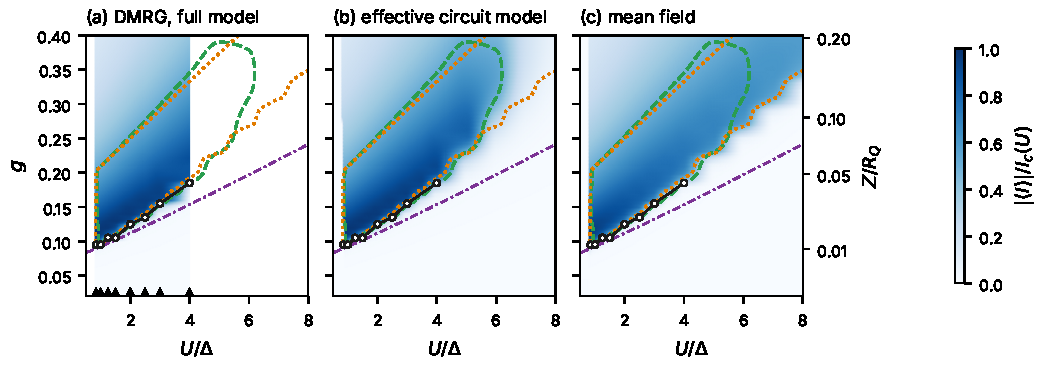
\includegraphics[width=\textwidth]{../figs/fig_phase_UG.pdf}
  \caption{\label{fig:phaseUG}%
  Phase diagram of the microscopic model~\eqref{eq:H} in the plane of the dot charging
  energy $U/\Delta$ and the mode coupling $g$ ($Z/R_Q=4g^2/\pi$, right axis), at
  $\hbar\omega=7.39\times10^{-4}\Delta$, $t_J=0.5\Delta$, $L=10$, no external flux
  (seed $\varphi_{\rm cl}=10^{-3}$). Colour: persistent current $|\langle I\rangle|$ from the
  gauge-invariant operator~\eqref{eq:Iop} in units of the junction critical current $I_c(U)$.
  (a) Full DMRG of electrons and photon (triangles: computed $U$ values; $g$ step $0.01$).
  (b) Effective circuit model $H_{\rm eff}$ with the DMRG $E(\varphi;U)$. (c) Mean field.
  Lines: contour $|\langle I\rangle|=0.5I_c$ from DMRG (solid), effective model (dashed) and
  mean field (dotted); white: classical threshold $\beta=1$.}
\end{figure*}

\begin{figure*}
  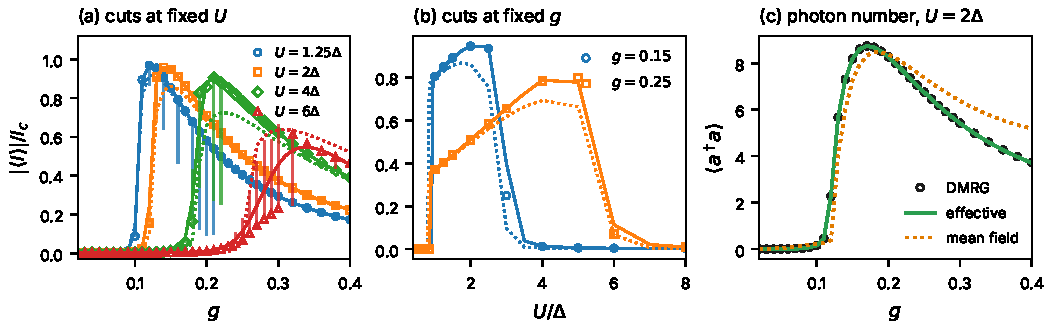
\includegraphics[width=\textwidth]{../figs/fig_phase_slices.pdf}
  \caption{\label{fig:phaseslices}%
  Cuts through Fig.~\ref{fig:phaseUG}. (a) Current versus $g$ at $U/\Delta=1.25,2,4$ and (b) versus
  $U$ at $g=0.15,0.25$: full DMRG (symbols), effective circuit model (solid), mean field (dotted).
  (c) Photon number at $U=2\Delta$.}
\end{figure*}

\begin{figure*}
  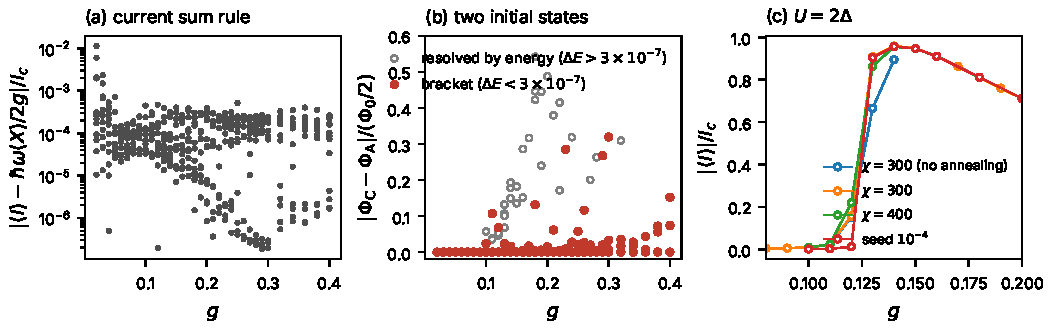
\includegraphics[width=\textwidth]{../figs/fig_phase_convergence.pdf}
  \caption{\label{fig:phaseconv}%
  Convergence of the full DMRG. (a) Violation of the sum rule~\eqref{eq:sumrule} over the whole
  grid. (b) Difference between the two initial states (vacuum side and polarized side) in units
  of $\Phi_0/2$. (c) $U=2\Delta$: bond dimension and seed dependence of the current near threshold.}
\end{figure*}
